\chapter{Motivating example}

\todo{Újracsinálni ezt az egészet, ez így egy okádék}

The target of this work is the runtime verification of distributed CPS systems. As a motivating example, the MoDeS3~\cite{modes3} demonstrator platform is used. 

 MoDeS3 stands for Model-based Demonstrator for Smart and Safe Systems. Its main goal is to demonstrate the many cool and innovative ways in which open source modeling tools can be used for systems development in the age of Internet-of-Things.
 
 The case study is a railway system: users can control trains arbitrarily as long as it is not dangerous. Accidents and dangerous situations are detected using sensors embedded into the track: they sense the trespass of the trains and send this information to the controllers. It is important to note that this is just local information, so we have to ensure that it will be shared between the components. The system employs six BeagleBone Black (BBB) embedded computers to run the safety logic, configured as a distributed system, where each BBB is responsible for some track sections.

\begin{figure}[H]
	\begin{center}
		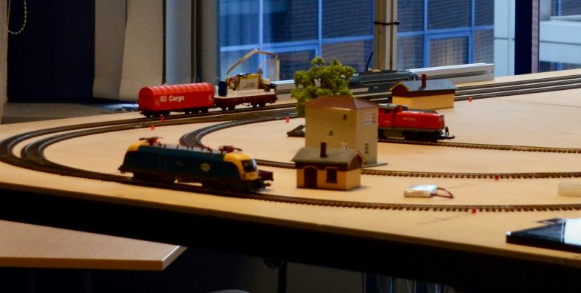
\includegraphics[width=\textwidth]{figures/modes.png}
	\end{center}
\end{figure}

\pagebreak
We use information from sensors perceiving the system's physical state to deduce if the state of the system is incorrect and/or dangerous. This is done by creating a structural model for the system and updating it based on sensor data coming from sensors. This model is graph based and we use graph pattern matching to find model parts indicating errors in the physical system.

Monitoring goals for this system are defined as graph patterns. The usage and efficiency of the developed framework are demonstrated by defining these goals, compiling them to monitoring codes and running them on variously distributed models. 



% célok és feladatok, amiket demonstrálni szeretnénk, monitoring goalok kiértékelése.S